% ADD/REMOVE THE 'answers' OPTION TO INCLUDE/SUPPRESS SOLUTIONS
% \documentclass[11pt,addpoints]{exam}
\documentclass[11pt,addpoints,answers]{exam}

\newcommand{\hwnum}{6}
\newcommand{\duedate}{February 25}

% In order to compile this file you will need to get 'header.tex'
% and make the line below point to the appropriate file path
\RequirePackage{microtype}
\RequirePackage{mathtools}
\RequirePackage{amsthm}
\RequirePackage{amssymb}
\RequirePackage{xspace}
\RequirePackage[shortlabels]{enumitem}
\RequirePackage{xcolor}
\RequirePackage{hyperref}
\RequirePackage[capitalize,nameinlink,noabbrev]{cleveref} % must load after hyperref
\usepackage{fvextra} % To use Verbatim
\RequirePackage[boxed]{algorithm}
\RequirePackage[noend]{algpseudocode}
\RequirePackage{tikz}

\hypersetup{breaklinks=true,
    colorlinks=true,
    linkcolor=blue,
    filecolor=blue,
    citecolor=blue,
    urlcolor=blue}

\algrenewcommand{\algorithmiccomment}[1]{\texttt{//} #1}
\algrenewcommand\algorithmicrequire{\textbf{Input:}}
\algrenewcommand\algorithmicensure{\textbf{Output:}}


% allow cleveref to label and reference enumerables defined in the exam class.
% these automatically define corresponding \Crefname as well.

% https://tex.stackexchange.com/questions/126020/cleveref-doesnt-use-correct-capitalized-name-if-used-with-amsthm
\makeatletter
\if@cref@capitalise
\crefname{question}{Question}{Questions}
\Crefname{partno}{Part}{Parts}
\crefname{subpart}{Subpart}{Subparts)}
\crefname{subsubpart}{Subsubpart}{Subsubparts}
\else
\crefname{question}{question}{questions}
\crefname{partno}{part}{parts}
\crefname{subpart}{subpart}{subparts}
\crefname{subsubpart}{subsubpart}{subsubparts}
\fi
\makeatother

% numeric sets in "blackboard" font

\newcommand{\N}{\mathbb{N}}
\newcommand{\Z}{\mathbb{Z}}
\newcommand{\R}{\mathbb{R}}
\newcommand{\Q}{\mathbb{Q}}
\newcommand{\C}{\mathbb{C}}
\newcommand{\Prop}{\mathbb{P}}

% paired delimiters

\DeclarePairedDelimiter\abs{\lvert}{\rvert}
\DeclarePairedDelimiter\length{\lVert}{\rVert}
\DeclarePairedDelimiter\norm{\lVert}{\rVert}
\DeclarePairedDelimiter\parens{(}{)}
\DeclarePairedDelimiter\tuple{(}{)}
\DeclarePairedDelimiter\brackets{[}{]}
\DeclarePairedDelimiter\floor{\lfloor}{\rfloor}
\DeclarePairedDelimiter\ceil{\lceil}{\rceil}
\DeclarePairedDelimiter\round{\lfloor}{\rceil}
\DeclarePairedDelimiter\set{\{}{\}}
\DeclarePairedDelimiter\inner{\langle}{\rangle}

\newcommand{\bit}{\set{0,1}}

% asymptotics

\DeclareMathOperator{\Otil}{\tilde{O}}
\DeclareMathOperator{\poly}{poly}
\DeclareMathOperator{\polylog}{polylog}
\DeclareMathOperator{\negl}{negl}

% algorithms

\newcommand{\algo}[1]{\textsc{#1}}

\newcommand{\memo}{\text{memo}}
\newcommand{\tabl}{\text{table}}
\newcommand{\backtrack}{\text{backtrack}}

\newcommand{\ALG}{\text{ALG}}
\newcommand{\OPT}{\text{OPT}}
\newcommand{\weight}{\text{weight}}
\newcommand{\val}{\text{value}}

% computability

% named language
\newcommand{\lang}[1]{L_{\text{#1}}}
% computational problem
\newcommand{\cproblem}[1]{\ensuremath{\text{#1}}\xspace}
% class of languages
\newcommand{\class}[1]{\ensuremath{\mathsf{#1}}\xspace}

\newcommand{\qst}{q_{\text{start}}}
\newcommand{\qacc}{q_{\text{acc}}}
\newcommand{\qrej}{q_{\text{rej}}}

\newcommand{\Lbarber}{\lang{BARBER}}
\newcommand{\atm}{\lang{ACC}}
\newcommand{\htm}{\lang{HALT}}
\newcommand{\ehtm}{\lang{$\varepsilon$-HALT}}
\newcommand{\eqtm}{\lang{EQ}}
\newcommand{\etm}{\lang{$\emptyset$}}
\newcommand{\epstm}{\lang{$\set{\varepsilon}$}}
\newcommand{\Lprop}{\lang{$\Prop$}}
\newcommand{\LSigmastar}{\lang{$\Sigma^*$}}

% complexity

\newcommand{\yes}{\ensuremath{\text{YES}}}
\newcommand{\no}{\ensuremath{\text{NO}}}

\newcommand{\DTIME}{\class{DTIME}}
\renewcommand{\P}{\class{P}}
\newcommand{\NP}{\class{NP}}
\newcommand{\NPH}{\class{NPH}}
\newcommand{\NPC}{\class{NPC}}
\newcommand{\coNP}{\class{coNP}}

\newcommand{\MAZE}{\cproblem{MAZE}}
\newcommand{\PALINDROME}{\cproblem{PALINDROME}}
\newcommand{\TSP}{\cproblem{TSP}}
\newcommand{\SAT}{\cproblem{SAT}}
\newcommand{\CSAT}{\cproblem{CSAT}}
\newcommand{\TSAT}{\cproblem{3SAT}}
\newcommand{\VC}{\cproblem{VERTEX-COVER}}
\newcommand{\SC}{\cproblem{SET-COVER}}
\newcommand{\HC}{\cproblem{HAMCYCLE}}
\newcommand{\HP}{\cproblem{HAMPATH}}
\newcommand{\IS}{\cproblem{IS}}
\newcommand{\CLIQUE}{\cproblem{CLIQUE}}
\newcommand{\SSUM}{\cproblem{SUBSET-SUM}}
\newcommand{\KNAPSACK}{\cproblem{KNAPSACK}}
\newcommand{\MAXCUT}{\cproblem{MAX-CUT}}

% randomness

\DeclareMathOperator*{\Var}{Var}
\DeclareMathOperator*{\Ex}{\mathbb{E}}

\newcommand{\RP}{\class{RP}}
\newcommand{\coRP}{\class{coRP}}
\newcommand{\BPP}{\class{BPP}}
\newcommand{\ZPP}{\class{ZPP}}
\newcommand{\BQP}{\class{BQP}}

%%% misc

\newcommand{\eps}{\varepsilon}

%%% theorems

\theoremstyle{plain}            % following are "theorem" style

\newtheorem{theorem}{Theorem}
\newtheorem{lemma}[theorem]{Lemma}
\newtheorem{corollary}[theorem]{Corollary}
\newtheorem{proposition}[theorem]{Proposition}
\newtheorem{claim}[theorem]{Claim}
\newtheorem{fact}[theorem]{Fact}
\newtheorem{openproblem}[theorem]{Open Problem}

\theoremstyle{definition}       % following are def style

\newtheorem{definition}[theorem]{Definition}
\newtheorem{conjecture}[theorem]{Conjecture}
\newtheorem{protocol}[theorem]{Protocol}
\newtheorem{exercise}[theorem]{Exercise}

\theoremstyle{remark}           % following are remark style

\newtheorem{example}[theorem]{Example}
\newtheorem{remark}[theorem]{Remark}
\newtheorem{note}[theorem]{Note}

%%% for homework and section notes

\newcommand{\commonheader}[2]{
    \pagestyle{headandfoot}
    \setlength{\headheight}{26pt}
    \setlength{\headsep}{16pt}

    \header
        {\small{\textbf{EECS 376: Foundations of Computer Science}} \\ \footnotesize{\textbf{University of Michigan, Winter 2025}}}
        {#1}
        {#2}

    \firstpageheadrule
    \runningheadrule

    \footer
        {}
        {\thepage}
        {}
}

\newcommand{\hwheader}{
    \commonheader
        {\Large \textbf{Homework \hwnum}}
        {\small \textbf{Due 8:00pm, \duedate\\ {\tiny(accepted until 9:59 pm, no credit after)}}}
}

\newcommand{\hwslnheader}{
    \commonheader
    	{}
        {\Large \textbf{Solutions to Homework \hwnum}}
    \printanswers
}

\newcommand{\notesheader}{
    \commonheader
    	{}
        {\Large \textbf{Discussion Notes \sectionnum}}
}

\newcommand{\practiceheader}{
    \commonheader
    	{}
        {\Large \textbf{Discussion Worksheet \sectionnum}}
}

\newcommand{\practiceslnheader}{
    \commonheader
    	{}
        {\Large \textbf{Solutions to Discussion Worksheet \sectionnum}}
}

\newcommand{\reviewheader}{
    \commonheader 
    \smallskip
    	{}
        {\Large \textbf{Midterm Review Notes}}
}

\newcommand{\hwpreface}{

\noindent This homework has \numquestions\ questions, for a total of \numpoints\ points and \numbonuspoints\ extra-credit points.

\noindent Unless otherwise stated, each question requires \emph{clear}, \emph{logically correct}, and \emph{sufficient} justification to convince the reader.

\noindent For bonus/extra-credit questions, we will provide very limited guidance in office hours and on Piazza, and we do not guarantee anything about the difficulty of these questions.
 
\noindent We strongly encourage you to typeset your solutions in \LaTeX.

\noindent If you collaborated with someone, you must state their name(s). You must \emph{write your own solution} for all problems and \emph{may not use any other student’s write-up}.
}

\newcommand{\hint}[1]{
\emph{Hint}: #1
}

% exam class setup
\pointsinmargin
\pointpoints{pt}{pts}
\bonuspointpoints{EC pt}{EC pts}
\marginpointname{ \points}
\marginbonuspointname{ \bonuspoints}


\usetikzlibrary{automata, positioning} % For TM
\newcommand{\lT}{\leq_T} % Turing reduces

\ifprintanswers
\hwslnheader   % header for solutions
\else
\hwheader   % header for homework
\fi

\begin{document}

\hwpreface

\begin{questions}
  \question[10] \textbf{Self assessment.} \nopagebreak
  
  Carefully read and understand the posted solutions to the previous homework.
  Identify one part for which your own solution has the most room for improvement (e.g., has unsound reasoning, doesn’t show what was required, could be significantly clearer or better organized, etc.).
  Copy or screenshot this solution, then in a few sentences, explain what was deficient and how it could be fixed.

  (Alternatively, if you think one of your solutions is significantly \emph{better} than the posted one, copy it here and explain why you think it is better.)

  If you didn't do last week's homework, choose a problem from it that looks challenging to you, and in a few sentences, explain the key ideas behind its solution in your own words.

  \begin{solution} 
  My answer for 3.b. lost points due to an incorrect explanation of the validity of OPT', and incorrect justification of why item (ii) implies that my algorithm is correct. My solution for 3.b. is as follows: 
  \begin{enumerate}[(i)]
    \item If $\ALG = \OPT$, then the algorithm is optimal. Otherwise, let $i_{\text{diff}}$ be the first index in $\ALG$ that is not in $\OPT$.\\
    Let $j$ be the first refill station in $\OPT$ occurring after the last common refill with $\ALG$, ($j=\OPT\{i_{diff}\}) $.
    \[
    \OPT' = (\OPT \setminus \{j\}) \cup \{i_{\text{diff}}\}.
    \]
    $\OPT'$ contains all indices $i_1, \ldots, i_{\text{diff}}$.

    \item
    Upon arriving at $i_{\text{diff}}$, the remaining water is insufficient to cover the next segment. Thus, refilling at $i_{\text{diff}}$ is necessary. Since any remaining water at $j$ would be without use in the event of a refill, replacing $j$ with $i_{\text{diff}}$ still provides a full bottle at the right time. Since this exchange involves only one station and does not change the total number of refills, $|\OPT'| = |\OPT|$, so $\OPT'$ is optimal.

    \item
    Since any optimal solution $\OPT$ can be transformed via $\ALG$ exchanges, it must be the case that $\ALG$ uses no more refills than $\OPT$. Therefore, the greedy algorithm $\ALG$ is correct.
  \end{enumerate}
  A correct solution for this problem might look like showing that because $i_{\text{diff}}$ is the vertex with the largest difference to $i_{\text{diff - 1}}$ such that the distance is less than $R$, $j < i_{\text{diff}}$, and then that the difference from $i_{\text{diff}}$ to the next vertex in OPT' (really, the next vertex in OPT) is at most $R$, and thus OPT' is valid. Also, it would employ an exchange argument to show that the algorithm is correct.
  \end{solution}

  \question \textbf{Turing machines warmup.} \nopagebreak
  
  Consider this \href{https://turingmachine.io/?import-gist=cb523cd1e010d4e02321f0cb2a8f6177}{Turing machine at turingmachine.io} (follow the link) over the input alphabet $\Sigma = \set{0, 1, \#}$ and tape alphabet $\Gamma = \Sigma \cup \set{\text x, \bot}$.
  Note that the site uses \textvisiblespace\ for the `blank' character, whereas we use $\bot$.
  
  \begin{parts}
    \part[2] Run the machine on the following input strings, and list all the ones it accepts. Fell free to simulate it on \href{https://turingmachine.io/?import-gist=cb523cd1e010d4e02321f0cb2a8f6177}{https://turingmachine.io/}. You do not have to justify your answer. 
    \begin{itemize}
        \item $\eps$
        \item $010$
        \item $10\#10$
        \item $100\#1$
        \item $101\#101$
        \item $110\#001$
    \end{itemize}
    
    \begin{solution} 
    \begin{itemize}
      \item 10\#10
      \item 101\#101
    \end{itemize}
    
    \end{solution}

    \part[4] State, with brief justification, what language the Turing machine decides, or that it does not decide any language.

    \begin{solution} 
    The Turing machine decides the language $\set{ w \# w : w \in \set{0,1}^* }$. For index $i$ in the string to the left of the \#, the machine removes \textsc{Left}($i$), and writes an x in the $i$th position in the string to the right of the \# if the characters at those positions are the same. If they are not the same, the machine rejects. If the result is a \# followed by a string of x's, the machine accepts. Otherwise, it rejects.
    \end{solution}

    \part[2] A \emph{bitwise complement} of a binary string is the result of flipping each bit, i.e., every $0$ is replaced with $1$ and vice versa. For example, the bitwise complement of $101$ is $010$. 
    
    Consider the following language:
    \[
        \lang{BIT-COMP} = \set{b\#\bar b: b \in \set{0,1}^* \text{ and $\bar b$ is the bitwise complement of $b$}}.
    \]

    Modify the transitions of the Turing machine above to decide $\lang{BIT-COMP}$. Include the screenshot of the modified Turing machine in your solution. You do not need to justify your answer.
    
    
    \begin{solution} 
    The modifications to the Turing Machine are making it so that if q3 sees a 0, it rejects, and if q4 sees a 1, it rejects. Also, if q3 sees a 1, it writes an x, and if q4 sees a 0, it writes an x. The modified Turing Machine is shown below:
    \begin{center}
      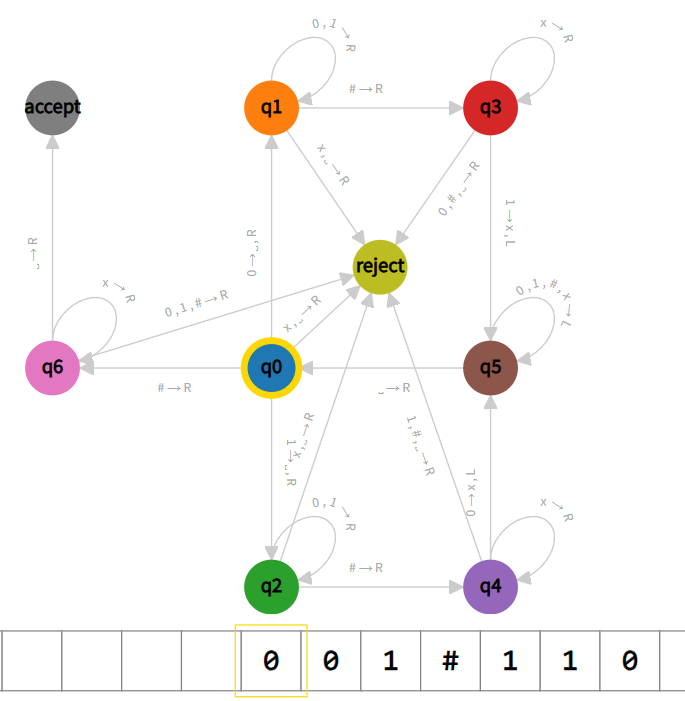
\includegraphics[width=0.8\textwidth]{hw6pr2c.png}
    \end{center}
    \end{solution}
    
  \end{parts}

  \pagebreak
  \question \textbf{Decidability and set operations.}\nopagebreak
    
  Let~$L$ be an \emph{undecidable} language over the alphabet $\Sigma$.
  Recall that this means the complement language~$\overline{L}$ is also undecidable, because we have shown that a language is decidable if and only if its complement is decidable.
  (In brief, the proof works by swapping the accept and reject states of any Turing machine that decides the language.)

  \begin{parts}
    \part[2]
    For each of following statements, give a \emph{decidable} language~$L_D$ that makes the statement true.

    (No justification is needed; the language $L_D$ can vary from one statement to the next.)
    
    \begin{enumerate}
    \item $L \cup L_D$ is decidable.
    \item $L \cup L_D$ is undecidable.
    \item $L \cap L_D$ is decidable.
    \item $L \cap L_D$ is undecidable.
    \end{enumerate}
    
    \begin{solution} 
    \begin{enumerate}
      \item Let $L_D = \Sigma^*$. Then, $L \cup L_D = \Sigma^*$ is decidable.
      \item Let $L_D = \varnothing$. Then, $L \cup L_D = L$ is undecidable.
      \item Let $L_D = \varnothing$. Then, $L \cap L_D = \varnothing$ is decidable.
      \item Let $L_D = \Sigma^*$. Then, $L \cap L_D = L$ is undecidable.
    \end{enumerate}
    \end{solution}
    
    \part[2]
    For each of following statements, give an \emph{undecidable} language $L_U$ that makes the statement true.
    
    (No justification is needed; the language~$L_U$ can vary from one statement to the next.)
    
    \begin{enumerate}
    \item $L \cup L_U$ is decidable.
    \item $L \cup L_U$ is undecidable.
    \item $L \cap L_U$ is decidable.
    \item $L \cap L_U$ is undecidable.
    \end{enumerate}
    
    \begin{solution} 
    \begin{enumerate}
      \item Let $L_U = \overline{L}$. Then, $L \cup L_U = \Sigma^*$ is decidable.
      \item Let $L_U = L$. Then, $L \cup L_U = L$ is undecidable.
      \item Let $L_U = \overline{L}$. Then, $L \cap L_U = \varnothing$ is decidable.
      \item Let $L_U = L$. Then, $L \cap L_U = L$ is undecidable.
    \end{enumerate}
    \end{solution}
    
  \end{parts}
  \pagebreak

  \question [6] \textbf{Undecidable within the infinite.}

  Prove, using diagonalization, that any \emph{infinite} language $L \subseteq \Sigma^*$ has an \emph{undecidable} subset.

  \hint{You may use the fact that any subset $T$ of a countable set $S$ is itself countable.}
  
  \begin{solution}
    Since $L$ is infinite, enumerate its elements as $w_1, w_2, w_3, \dots$. \\
    Let $\{M_1, M_2, M_3, \dots\}$ be an enumeration of all deciders for decidable languages. \\
    Define:
    \[
    L' = \{\,w_i \in L \mid M_i \text{ does not accept } w_i\,\}.
    \]
    Assume, for contradiction, that $L'$ is decidable by some decider $M_k$. Then
    \begin{align*}
      w_k &\in L' \iff M_k \text{ does not accept } w_k \\
      w_k &\notin L' \iff M_k \text{ accepts } w_k.
    \end{align*}
    Based on the definition of $M_k$ being a decider for $L'$, if $w_k$ is in $L'$, then $M_k$ should accept $w_k$, and if $w_k$ is not in $L'$, then $M_k$ should not accept $w_k$. This does not happen, and thus is a contradiction. \\
    Therefore, $L'$ is undecidable.
  \end{solution}

  \ifprintanswers
  \else
  \pagebreak
  \fi

  
\medskip \hrule \medskip 
\emph{\cref{halt-alt} through \cref{loop-n-loop} contain content covered in Lecture 11 on 2/17.}

\emph{Reminder: Turing machines are computationally equivalent to computer programs, so treat ``give a Turing machine" as ``give an algorithm," except possibly providing a halting analysis instead of a runtime analysis when necessary.}

\medskip \hrule \medskip

  \question [8] \textbf{Alternative $\htm$ undecidability.}  \label{halt-alt}
  
  \nopagebreak

  Recall the language
  \[
        \htm = \set{(\inner{M},x): \text{$M$ is a TM and $M$ halts on $x$}} \text .
  \]
  
  In this problem, you will derive a proof that $\htm$ is undecidable without relying on the undecidability of any other language.
  This was the first existence proof for an undecidable language, and it is due to Alan Turing.

    
Suppose for the sake of contradiction that some Turing machine $H$ decides $\htm$. Give and analyze a Turing machine $B$ which takes (the description of) a Turing machine as input, and has access to $H$ as an oracle, that shows that the original  hypothesis (that $\htm$ is decidable) must be false.

    \hint{A Turing machine may be designed to loop indefinitely.}

    \begin{solution}
    Turing machine $B$, on input $\langle M \rangle$, operates as follows:
    \begin{enumerate}
        \item Run $H$ on the input $(\langle M \rangle, \langle M \rangle)$.
        \item If $H$ accepts ($M$ halts on $\langle M \rangle$), then loop indefinitely.
        \item If $H$ rejects ($M$ does not halt on $\langle M \rangle$), then halt.
    \end{enumerate}
    Consider the behavior of $B$ on its own description $\langle B \rangle$:
    \begin{itemize}
        \item If $B(\langle B \rangle)$ halts, then $H$ must have rejected on $(\langle B \rangle, \langle B \rangle)$, implying that $B(\langle B \rangle)$ does not halt.
        \item If $B(\langle B \rangle)$ does not halt, then $H$ must have accepted on $(\langle B \rangle, \langle B \rangle)$, implying that $B(\langle B \rangle)$ halts.
    \end{itemize}
    In both cases, a contradiction is reached, and therefore, the assumption that $\htm$ is decidable must be false.
    \end{solution}

  \question \textbf{Turing reduction warmup.} \label{prob:decidablity} \nopagebreak
  
  \begin{parts}

    \part[4] Prove or disprove: Every language is Turing-reducible to its complement, i.e., $L \lT \overline{L}$ for any language $L$.

    \begin{solution} \end{solution}
    
    \part[4] Prove or disprove: A decidable language is Turing reducible to any language, i.e., $L \lT L'$ for any decidable language $L$ and any language $L'$. 

    (A disproof could consist of specific languages $L, L'$ and a proof that the statement does not hold for them.)
    
    \begin{solution} \end{solution}
    
    \part[4] Prove or disprove: let~$L$ be a language; if there exists a language~$L'$ such that $L \lT L'$, then $L$ is decidable.

    (A disproof could consist of specific languages~$L$ and~$L'$ where $L \lT L'$ but~$L$ is undecidable.)

    \begin{solution} \end{solution}
  \end{parts}

\medskip \hrule \medskip
    \emph{If you haven't already, please read \href{https://drive.google.com/file/d/1hryh8KKZmLlzNPIej31PHR1QkcNAKx9D/view}{Handout 5: Turing Reductions} and apply it in your solution for the next few problems.}
\medskip \hrule \medskip
  

  \question \textbf{Professor $\Upsilon$'s reductions.} \nopagebreak

  Professor~$\Upsilon$ has given you several statements and claimed proofs concerning Turing reductions, but every claimed proof has one major logical error!
  Identify and briefly explain each of these errors. You do not need to repair the proofs when that's possible, nor determine whether the statements are actually true, though these are good exercises too!
        
  \begin{parts}
    
    \part[5] \textbf{Statement:} Let $A = \set{0^k 1^k: k \ge 0}$ over $\Sigma = \set{0,1}$, and let $B = a^* b^*$ over $\Sigma = \set{a,b}$.
    Then~$A$ Turing-reduces to $B$.
        
    \textbf{Claimed Proof:} Let $D_B$ be an oracle that decides $B$.
    Consider the following Turing machine $D_A$ that has access to $D_B$.

    \begin{center}
      \begin{minipage}{0.8\linewidth}
        \begin{algorithm}[H]
          \begin{algorithmic}[1]
            \Function{$D_A$}{$x$} \Comment{$x = x_1 x_2 \cdots x_n$}
            \For {$i=1, \ldots, n$}
            \If {$x_i = 0$} {$w_i \gets a$}
            \Else { $w_i \gets b$}
            \EndIf
            \EndFor
            \State \Return $D_B(w)$
            \EndFunction
          \end{algorithmic}
        \end{algorithm}
      \end{minipage}
    \end{center}
    
    Clearly, $D_A$ halts on any input because~$x$ has finite length, and $D_B$ halts on any input by assumption.
    By the definitions of~$A$ and~$B$, the code of $D_A$, and the hypothesis on $D_B$,
    \begin{align*}
      x \in A &\iff w \in \set{a^k b^k : k \ge 0} \\
              &\iff w \in B \text{ (since `star' means ``zero or more'')} \\
              &\iff D_B(w) \text{ accepts} \\
              &\iff D_A(x) \text{ accepts.}
    \end{align*}
    So, we have shown that $D_A$ decides $A$, and hence $A \lT B$. 
    
    \begin{solution} \end{solution}
    
    \part[5]
    \textbf{Statement:} $\atm$ Turing-reduces to \emph{any} language~$L$ where $L \neq \emptyset$ and $L \neq \Sigma^*$.
    
    \textbf{Claimed Proof:}
    Let~$L$ be any such language and let $D_L$ be an oracle that decides $L$.
    Consider the following Turing machine $D_A$ that has access to $D_L$. 
    
    \begin{center}
      \begin{minipage}{0.8\linewidth}
        \begin{algorithm}[H]
          \begin{algorithmic}[1]
            \Function{$D_A$}{$\inner{M},x$}
            \If {$M(x)$ accepts}
            \State let $w$ be an arbitrary string in $L$
            \Else
            \State let $w$ be an arbitrary string not in $L$
            \EndIf
            \State \Return $D_L(w)$
            \EndFunction
          \end{algorithmic}
        \end{algorithm}
      \end{minipage}
    \end{center}
    By the definition of $\atm$, the code of $D_A$, and the fact that $D_L$ decides~$L$, we have that
    \begin{align*}
      (\inner{M},x) \in \atm
      & \iff M(x) \text{ accepts } \\
      & \iff w \in L  \\
      & \iff D_L(w) \text{ accepts} \\
      & \iff D_A(\inner{M},x) \text{ accepts}.
    \end{align*}
    Thus, $D_A$ decides $\atm$, hence we have shown that $\atm \lT L$.
    
    \begin{solution} \end{solution}
  \end{parts}
    
  \question \textbf{Loop and loop.} \label{loop-n-loop}
  \nopagebreak
  
  \begin{parts}
  
    \part[6] Define \[ \lang{AND-LOOP} = \set{(\inner{M},x,y) : M \text{ is a TM that loops on input $x$ and loops on input $y$}} \; \text.
    \] Prove that $\htm \lT \lang{AND-LOOP}$.
    Note that since $\htm$ is undecidable, this means that $\lang{AND-LOOP}$ is undecidable.
    
    \begin{solution} \end{solution}

    \part[6] Define \[\lang{SELF-LOOP} = \set{\inner{M} : M \text{ is a TM that loops on input } \inner{M}} \text.\] Prove that $\Lbarber \lT \lang{SELF-LOOP}$.
    Note that because $\Lbarber$ is undecidable, we can conclude $\lang{SELF-LOOP}$ is undecidable.

    \begin{solution} \end{solution}

\end{parts}

\medskip \hrule \medskip 
\emph{\cref{finite-n-finite} and \cref{tr} contain content covered in Lecture 12 on 2/19.}
\medskip \hrule \medskip

\question \textbf{Finite and finite.}\label{finite-n-finite}

  \label{finite}
  
  For each of the following languages, determine whether it is decidable. If it is decidable, describe and analyze a Turing machine that describes it. Otherwise, prove its undecidability by reducing a known undecidable language to it.


\begin{parts}
    
    \part[6] Let $\lang{I'M-FINITE} = \set{\ell_1, \ldots, \ell_n}$ be a finite language, i.e., a language containing only a finite number of strings. \label{I'M-FINITE}
    
    Determine, with proof, if $\lang{I'M-FINITE}$ is decidable.
    
    \begin{solution} \end{solution}

    \part [8] Define the language 
    \[
        \lang{FINITE} = \set{ \inner{M} : M \text{ is a TM and $L(M)$ is finite} } \text .
    \] 
    Determine, with proof, if $\lang{FINITE}$ is decidable.
    
    \begin{solution} \end{solution}
    
\end{parts}


  \question \textbf{Turing reductions.} \label{tr}

  For each of the following languages, show that it is undecidable via a Turing reduction from a language we have already shown is undecidable.

  \begin{parts}
    \part[8] $\lang{SUBSET} = \set{(\inner{M_1}, \inner{M_2}) : M_{1}, M_{2} \text{ are TMs and } L(M_1) \subseteq L(M_2)}$. 

    \hint{You may call an oracle multiple times.}
    
    \begin{solution} \end{solution}

 \part [8] $\lang{FASTER} = \set{(\inner{M_1}, \inner{M_2}, x) : M_1(x) \text{ runs for strictly fewer steps than } M_2(x) \text{ does}}$.

    \hint{A computation that halts takes strictly fewer steps than one that loops.
    If both computations loop, then neither takes strictly fewer steps than the other.}
    
    \begin{solution} \end{solution}
  
  \end{parts}

  \bonusquestion \textbf{Goldbach conjecture (optional extra credit).} 
  
  The \emph{Goldbach Conjecture} states that every even integer greater than two is the sum of two primes.
  For example, $20=7+13$, $22=3+19$, $24=5+19$, etc. The conjecture has been confirmed for all even integers up to about $4 \times 10^{18}$, but no proof or counterexample is known; resolving the conjecture is one of the oldest unsolved problems in mathematics.

  In this problem, you will show that if we had a ``magic box'' (an oracle) that decides $\htm$, then we would have an algorithm that determines whether the Goldbach Conjecture is true!
  More generally, an oracle for $\htm$ would let us resolve many open questions in mathematics.

  \begin{parts}
    \bonuspart [2] Consider the language
    \[
        \lang{GOLDBACH} = \set{x \in \N: \text{$\forall y > x$, $2y$ is the sum of two primes}}
    \]
    State, with brief justification, whether $\lang{GOLDBACH}$ is decidable.

    \begin{solution} \end{solution}
    

    
    \bonuspart [2]
    Let $H$ be an oracle that decides $\htm$.
    Give a Turing machine $M_G$ that has access to $H$ and, on any input, accepts if the Goldbach Conjecture is true, and rejects otherwise.

    \hint{First construct a Turing machine that halts if and only if the Goldbach Conjecture is false. You may use a function $\algo{isPrime}$ that returns whether a given number is prime (a Turing machine can do this).} \label{Goldbach-a}
    
    \begin{solution} \end{solution}


    \bonuspart [1]
    Now consider the language
    \[ 
        \lang{SMALL-HALT} = \set{(\inner{M},x) : M \text{ is a TM, } M(x) \text{ halts, and } (\inner{M},x) \text{ has $< 1000$ characters}} .
    \] 
    
    We asserted in class that this language is decidable, i.e., some TM~$M_{SH}$ decides it.

    Briefly explain whether your solution from \cref{Goldbach-a} still works if you replace the oracle~$H$ with the Turing machine~$M_{SH}$---if so, this would yield an ordinary Turing machine (with no oracle) that, when run on any input, would tell us whether the Goldbach Conjecture is true! 
    
    \emph{Food of thought: If your answer is `yes', why hasn't anyone prove or disprove the Goldbach Conjecture?}
      
    \begin{solution} \end{solution}

  \end{parts}
  
\end{questions}

\end{document}
